\documentclass[main.tex]{subfiles}

\begin{document}


\section*{Appendix}

\begin{figure}[H]
\centering
\caption{Co2 Emissions}
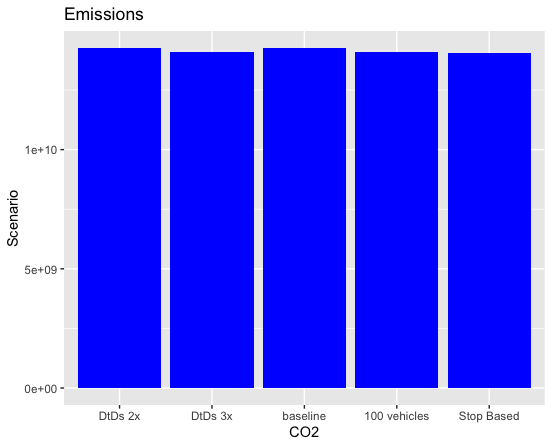
\includegraphics[width=10cm]{images/Co2_new.png}
  \label{fig:15}
\end{figure}

\begin{figure}[H]
\centering
\caption{NOx Emissions}
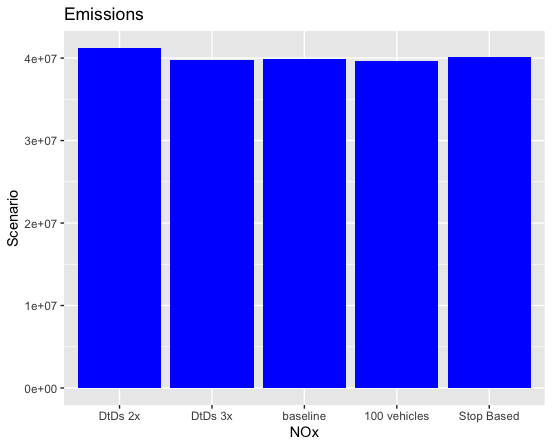
\includegraphics[width=10cm]{images/Nox_new.png}
  \label{fig:16}
\end{figure}

The basis of an agent-based MATSim simulation is a synthetic population of the case study area. For Switzerland, a range of rich
data sources are available that make it possible to set up such a population with detailed socio-demographic and behavioral attributes.
In the following, the process will be described in brief. A more detailed description of the Swiss data sets and how they have been
processed can be found in (H¨orl, 2020). Furthermore, (H¨orl and Balac, 2020) describes the methodology in detail for the case of Paris
and ˆIle-de-France. There, unlike Switzerland, all necessary data sets are publicly and openly available to replicate the process.
Initially, the synthetic Swiss population is based on the STATPOP data set, which is a comprehensive census of Switzerland,
including attributes like age and gender of all residents, but - most notably - also location by coordinate of each household. Persons and
households from this data set are used directly as a basis of the Swiss synthetic population. Afterward, work or educational locations for
each synthetic person are added. For that, the Structural Survey is used, which, unlike the registration-based census data, is a detailed
household survey conducted for around 3% of the Swiss population each year. From this data set, an origin–destination matrix between
home and work/education municipalities in Switzerland can be derived, then used to proportionately sample destination zones for
each agent, based on their home zone. In the third step, the national Mobility and Transport Microcensus is employed: a classical
household travel survey providing full day activity patterns for around 60,000 respondents. We use a statistical matching procedure to
sample and attach activity chains to the synthetic persons, based on socio-demographic attributes. This way, activity patterns
correlating with certain age groups or gender are assigned according to the population. These activity chains contain activity types,
activity durations and connecting modes of transport as reported in the survey data. As departure and arrival times are rounded
strongly (in five minute intervals) as is the case in many surveys, activity chains (including all departure and arrival times) are shifted
by a random offset of +/- 30 min for each person to avoid having unrealistically many people departing at the same time at one
location, which would, in turn, affect the traffic dynamics in the simulation negatively. Finally, specific work and education locations
are sampled, based on the destination zones of the agents, from STATENT, the national enterprise census, which lists all facilities in
Switzerland by coordinate. Further, secondary activities in the agents’ plans (such as shopping or leisure), are assigned to discrete
facilities using a specifically-designed algorithm for secondary location assignment (H¨orl and Axhausen, 2020). To complete the
simulation data, an exhaustive digital public transit schedule for Switzerland is integrated into the simulation and the road network is
extracted from OpenStreetMap, including all roads from motorways to residential roads. In total, this process yields a synthetic
representation of Switzerland that reproduces the daily mobility needs of the population and available infrastructure.


Note that MATSim, in
principle, is also able to consider departure time choices or even location choice through its co-evolutionary algorithm, which is a
different process of decision-making not used here; our goal was to directly integrate a discrete choice model into MATSim. Unlike the
standard approach, it inherently contains consistent information about the trade-offs people make between choice dimensions when
faced with the automated mobility option. The standard co-evolutionary algorithm would only allow us to perform sensitivity analyses
on the relatively unspecific attractively level of the new transport mode.Due to the complexity of the simulation, the dense network and the large number of agents, we restrict simulations to 10\% samples
of the population, with road capacities being scaled down accordingly


We use a statistical matching procedure to sample and attachactivity chains to the synthetic persons, based on socio-demographic attributes. This way, activity patternscorrelating with certain age groups or gender are assigned according to the population. These activity chainscontain activity types, activity durations and connecting modes of transport as reported in the survey da

For the simulation of mobility behaviour we utilise the multi-agent transport simulation framework MATSim version 14.0 \citep{Horni.2016}. A synthetic scenario of Cape Town with a population sample size of 10\,\% is employed for the study. We derive the synthetic population from South African Census Data 2011 \citep{census2011}, the 10\% Public Use Sample \citep{census2011public10pct} and the Minnesota Population Center Integrated Public Use Microdata Series \citep{mpc2020}. For the population synthesis process we employ a mlti-level iterative proportional fitting methodology \citep{joubert2014mipf}. Furthermore, we utilize data from National Household Travel Survey 2013 \citep{nhts2013} and the Time Use Survey 2010 \citep{tus2013} to assign individual mobility behaviour to the synthetic agents.  \\

On the supply side we employ network and infrastructure data from OpenStreetMap (OSM) \citep{osm}. The network links are downscaled according to the population sample in terms of flow and storage capacities. Furthermore, the individual OSM ids of the dataset are extracted and categorised into different activities such as "shopping" or "leisure". In addition, we use GTFS datasets from the main public transport providers in Cape Town from 2018 to model public transport \citep{transifeeds}. The capacities of the vehicles are also downscaled according to the population sample, as the adjustment of the vehicle size to the downscaled network leads to a distortion of the passenger flows. To avoid further distortions in the timetables of the vehicles by the other network participants and for reasons of simplification, the vehicles of Golden Arrow Bus Services (GABS), Metrorail Western Cape, MyCiTi Cape Town Integrated Rapid Transit (IRT) system and UCT campus shuttle buses (Jammie) operate on a pseudo-network with direct aerial lines between stops and with adjusted speed limits on each route to match the timetable. For the modelling of informal public transport in the form of minibus taxis, the use of a pseudo-network is omitted due to the fact that the number of minibus taxis is significantly higher than in the case of formal public transport which leads to feedback effects in the traffic flow. To represent these effects in the overall traffic in Cape Town the Minibus Taxis travel together with the other individual traffic on the OSM motor roads.\\

Again, using the OSM data, the modelled infrastructure and the socio-demographic characteristics of the agents such as age, gender and employment status, a gravity model is used to create a path-destination matrix and assign it to the agents. The resulting base population then goes through several calibration steps, calibrating towards NHTS averages and Cape Town Vehicle Detection System (VDS) traffic flow data on major roads from 2018. The calibration target is set at an average deviation from real data of less than 20\% error for car traffic and less than 50\% for formal and informal public transport.\\

\end{document}